%!TEX root = JournalChapter1.tex
\section{Investigating Retrieval Model Problems}
\label{RMinvestigation}
The literature has identified \textbf{document length normalization} as the main culprit for the under-performance of retrieval efforts in microblogs. The work by \cite{naveed2011searching} suggests that the \textbf{Verbosity} and \textbf{Scope} hypotheses do not hold for microblog retrieval. The \textbf{verbosity} hypothesis supports that some authors are more verbose than others, and hence applying length normalization by dividing by the length of the document is beneficial to better capture relevance, as repetition of terms is superfluous. On the other hand, the \textbf{scope} hypotheses states that some authors simply have more to say, thus naturally adding more relevant information to the topic. As a result documents are longer but more extensive and rigorous in their content than shorter ones. The added value of longer documents should be accounted for and thus promoted over shorter ones.

In the context of Microblog retrieval, \cite{naveed2011searching} carried out a number of experiments using a logistic regression model over a number of tweet features as the retrieval methodology. They showed significant improvements in performance when their algorithm did not perform document length normalization over its normalised counterpart. However, since in their work their ranking approach takes into consideration multiple other features, it is not clear if their finding about document length normalization is generalisable.

Furthermore, although it is been often assumed, it is not known if length normalisation is bad altogether for microblog retrieval, or maybe is just how it is interpreted in this particular case what makes it harmful. Intuition tell us that document length normalization as we know it does not interact well with the limitations characterised by microblogs. The \textbf{Verbosity} and \textbf{Scope} hypotheses seem not to model the behaviour of users publishing microblogs. Microblog users generally have the challenge of fitting their messages within the strict character limit. Consequently, retrieval models designed under scope and verbosity or similar premises, such as BM25 \cite{robertson2009probabilistic} are likely to exhibit unexpected behaviour, as it can be observed in Tables \ref{traditional}.

To aid in developing our understanding of the behaviour of retrieval models we formalise their composition. To this end we have compiled Table \ref{modelfeatures} to show the different components involved in the score computation of a variety of state of the art retrieval models. The top row of the table indicates whether the component relies on collection statistics (I.e. Collection feature) or the document itself (Document feature). The second row contains acronyms for each of the features, which are expanded as: 

\begin{itemize}
\item [ADL.] \textbf{AverageDocumentLength:} This is the average document length, in number of tokens, for the whole collection.
\item [DL.] \textbf{DocumentLength:} This is the document length, in number of tokens, for the document being scored.
\item [ND.] \textbf{NumberOfDocuments:} Total number of documents in the collection. 
\item [DF.] \textbf{DocumentFrequency:} Number of documents in which the term appears (I.e. A term's posting list size).
\item [NT.] \textbf{NumberOfTokens:} Number of different tokens in the collection.
\item [CTF.] \textbf{CollectionTermFrequency:} Frequency of a term in the whole collection. (I.e. Total number of occurences of a term in the collection)
\item [TF.] \textbf{TermFrequency:} Frequency of the term in the document being evaluated.
\end{itemize}

\begin{table}[]
	\caption{Features involved in the computation of retrieval models.}
	\centering
	\begin{tabular}{|l|c|c|c|c|c||c|c|} 
		\cline{2- 8}
		\multicolumn{1}{c|}{}& \multicolumn{5}{c||}{Collection Features} &  \multicolumn{2}{c|}{Document Features} \tabularnewline
		\cline{2- 8}
		\multicolumn{1}{c|}{}
		& \textit{\textbf{ND} } & \textit{\textbf{DF} } & \textit{\textbf{ADL} } & \textit{\textbf{NT} } 
		& \textit{\textbf{CTF} } & \textit{\textbf{TF} } & \textit{\textbf{DL} } \tabularnewline \hline
		\textit{IDF} 	& * &  *&  	&   &  	&	&   \tabularnewline \hline
		\textit{DFRee} 	&   &   &   & * & * &*	&* \tabularnewline \hline
		\textit{BM25}	& * &  *& * &   &  	&*	&* \tabularnewline \hline
		\textit{HLM} 	&   &   &  	& * & * &*	&* \tabularnewline \hline
		\textit{DLM} 	&   &   &  	& * & * &*	&* \tabularnewline \hline
	\end{tabular}
	\label{modelfeatures}
\end{table}

Each of the remaining rows contain the name of the retrieval model as well as whether a component involved in its computation (Denoted by *). For example, DFRee uses NumberOfTokens (NT), CollectionTermFrequency (CTF), TermFrequency (TF) and Document Length (DL).

In the following sections we investigate the behaviour of the abovementioned retrieval models in terms of these features. We perform our analysis mainly by means of simulating their behaviour with a range of different values common under microblog retrieval conditions.

\subsection{The BM25 Case}
\label{bm25case}
The work by \cite{ferguson2012investigation} examined the performance of BM25 when used under a microblog retrieval scenario. Their findings showed how the closer to zero the free parameters were set in BM25, the better the performance achieved. However, they did not connect this finding to the design of BM25 and what these settings meant in terms of the affected components. In this section we exemplify and connect these findings to the theory by simulating the behaviour of BM25 under microblog retrieval conditions.

% and examine how they affect other retrieval models aside from BM25.
First, we observe in Table \ref{modelfeatures} how BM25 relies on document length by using both ADL and DL components in its computation. Furthermore, BM25 has two free parameters, namely \(b\) and \(k_1\), which control the effects of the ``saturation function'' over the final score. The saturation function in BM25 encodes the document length evidence as part of the score as follows: 

The first version of the saturation function is given by:

\begin{equation}
 \text{Version 1: }\frac{f(q_i, D)}{f(q_i, D) + k_1} \text{   for some k_1 $>$ 0}
\end{equation}

Once we take into consideration the Verbosity and Scope hypotheses, the following saturation function can be derived:

\begin{equation}
 \text{Version 2: }\frac{f(q_i, D)}{f(q_i, D) + k_1*((1-b)+b*dl/avdl)} \text{   for some k_1 $>$ 0}
\end{equation}

The main difference between these equations is that \textbf{Version 2} reduces the effect of term frequency with respect to the document length and its collection average, whilst \textbf{Version 1} only relies on the \(k_1\) free parameter. Secondly, the free parameter \(b\) ponders between the Verbosity and Scope hypotheses. Setting \(b\) to 0 effectively disables the Verbose hypothesis, giving full weight to Scope, in other words, the longer the document the better. Thus when \(b\) is set to 0, \textit{Version 2} of the saturation function becomes \textit{Version 1}.

As we mentioned before, the study carried by \cite{ferguson2012investigation} explored the best parameters for \(b\) and \(k_1\) concluding that best performance is achieved as both parameters tend to 0. However, the authors did not mention is that by setting those parameters close to 0, we are disregarding the document length normalisation component altogether. Thus for all intents and purposes BM25 becomes IDF. This can be proved mathematically by substituting \(b\) and \(k_1\) by 0 as follows \ref{bm25proof}.

\begin{small}
\begin{align}
\label{bm25proof}
    \notag \text{BM25}(D,Q) &= \sum_{i=1}^{n} \text{IDF}(q_i) \cdot \frac{f(q_i, D) \cdot (k_1 + 1)}{f(q_i, D) + k_1 \cdot (1 - b + b \cdot \frac{|D|}{\text{avgdl}})} \\
  \notag&= \sum_{i=1}^{n} \text{IDF}(q_i) \cdot \frac{f(q_i, D) \cdot (0 + 1)}{f(q_i, D) + 0 \cdot (1 - 0 + 0 \cdot \frac{|D|}{\text{avgdl}})} \\
  \notag&= \sum_{i=1}^{n} \text{IDF}(q_i) \cdot \frac{f(q_i, D)}{f(q_i, D) } \\
  &= \sum_{i=1}^{n} \text{IDF}(q_i)              
\end{align}
%\end{proof}
\end{small}

Initially it would seem that the \textbf{Scope} and \textbf{Verbosity} hypotheses do not hold for microblogs. The reasoning behind being that these hypotheses were developed for documents that were unbounded in terms of their length such as web pages or books. However, since document length has an upper bound in microblogs, authors express their ideas in a very constrained space where verbosity and scope hypotheses do not seem to hold. However we will later observe that this conclusion is partially true\footnote{We later demonstrate that \textbf{scope} does hold, but not \textbf{verbosity}}.

\begin{figure}[]
  \centering
   \include{bm25TFDL}
     \caption{Term Frequency (TF) vs, Doc. Length (DL)}
  \label{bm25scoretfdl}
\end{figure}

Furthermore, terms in microblog documents have very low document frequencies and more often than not, query terms appear at most once in each document unless dealing with spam. Thus a query term appearing more than once within a document can have a dramatic effect over the score produced by BM25. In other words, the very low document frequencies result in unreliable estimations of the informativeness of a query term. Consequently, in this particular case, it is better to rely on features outside the document such as collection features.

Finally, Figure \ref{bm25scoretfdl} shows the possible BM25 scores for a range of Term Frequency (TF) and Doc. Length (DL) values.\footnote{Where \(ND=100k\) and \(DF=100\)}. We can extract two interesting behaviours which we can compare later to other retrieval models. Firstly the increase of document length is regarded as negative. In other words the more information in number of terms is encoded in the document the less relevant it is regarded. Secondly the increasing term frequency results in increased scores. This would seem counter-intuitive in a document with such a limited length, as users normally struggle to fit their messages. Additionally, there is a danger of promoting spam messages which may only contain the query terms.


%\mentalnote{Finally, by reducing the values of the b and k constants, the standard deviation of across the scores (w.r.t. tf and dl) by bm25 is also reduced, reaching 0 when b and k are 0, as tf and dl do not play any role in this case. Lower stdev. better performance}

\subsection{The Hiemstra's Language Model (HLM) Case}
In this section we study the Hiemstra's Language Model (HLM) \cite{hiemstra2001using} under Microblog conditions. Table \ref{modelfeatures} shows that HLM utilises both CollectionTermFrequency (CTF) and TermFrequency (TF) together with the total number of different tokens in the collection (NT) and document length (DL). Furthermore, if we pay attention to Table \ref{traditional} we can observe that whilst DFR and HLM utilize the same components, HLM exhibits a more erratic performance under microblog conditions. HLM's performance for the 2013 collection is considerably lower than that of DFR or IDF, whereas it remains close to the top performing models for the 2011, 2012 and 2014 collections. Let us look into the formulation of HLM: 

\begin{small}
\begin{align}
\label{hlmformula}
    \text{HLM}(D,Q) &= \sum_{i=1}^{n} \log_2 \left[ 1 + \frac{c \cdot f(q_i, D) \cdot ntoks }{ (1-c) \cdot f(q_i, C) \cdot |D|} \right]
\end{align}
\end{small}

where $ntoks$ refers to the number of unique tokens in the collection (NT), $c$ is a free parameter, and $C$ represents the set of all documents in the collection. $f(q_i, D)$ represents the TF of a query term $q_i$ in document $D$, whereas $f(q_i, C)$ is CTF of term $q_i$. The free parameter c regulates how HLM satisfies the conditions of \textbf{coordination level ranking (CLR)}) \cite{hiemstra2000relating}. CLR is a rule enforced in the design of HLM which ensures that documents containing $n$ query terms are ranked higher than those with $n-1$ terms.

Similarly to BM25, the assumption where higher term frequencies should be regarded positively, can easily result in the promotion of spam and undesired results. And this is rooted in the fact that query terms occur normally 1-2 times in a microblog document, due to length limitations.

%\begin{figure}[]
%%        
%%       \begin{subfigure}[b]{0.5\textwidth}
%%        \centering
%%        \caption{Doc. Frequency (CTF) vs, $c$}
%%         \input{hlmfigure-df-c}
%%      \end{subfigure}      
%%      ~
%       \begin{subfigure}[b]{0.5\textwidth}
%        \centering
%        \caption{Doc. Frequency (CTF) vs, Doc. Length (DL)}
%         \input{hlmfigure1}
%		\label{hlm-ctf-dl}
%      \end{subfigure} 
%    \caption{HLM analysis}
%		\label{hlmanalysis}
%\end{figure}

%\begin{figure}[]
%	\centering
%	\caption{HLM: Doc. Frequency (CTF) vs, Doc. Length (DL)}
%	\input{hlmfigure1}
%	\label{hlm-ctf-dl}
%\end{figure} 

\begin{figure}[]
     \begin{subfigure}[b]{0.5\textwidth}
      \centering
      \caption{TF vs, Doc. Length (DL)  with $c = 0.15$}
       \input{hlmfigureDLVSTF}
       	\label{cTFVSDL15}
    \end{subfigure}  
      ~
     \begin{subfigure}[b]{0.5\textwidth}
      \centering
      \caption{TF vs, Doc. Length (DL)  with $c = 0.99$}
       \input{hlmfigureDLVSTF99}
       \label{cTFVSDL99}
    \end{subfigure}  
    \caption{HLM analysis}
	\label{cTFVSDL}
\end{figure}

%Figure \ref{hlm-ctf-dl} shows HLM scores with respect to ``collection term frequency (CTF)\footnote{Also known as ``document frequency''}'' and document length (DL). 
Figure \ref{cTFVSDL15} shows a plot of the possible scores produced by HLM in its default configuration (\(c=0.15\))\footnote{Where \(ND=100k\), \(DF=100\) and \(NT=1000\)}. We can observe that for documents where the length is lower than 5 the differences between the scores are very marked. Above length 5 the progression of scores is much more subtle. In other words, shorter documents are subject to high differences between their scores due to small changes in their limited length.

Furthermore, we can observe in Formula \ref{hlmformula}, how the high sensitivity to low document length is a result of the model's design, since document length acts as a multiplier in the denominator. Additionally, term frequency can be found within the nominator as a multiplying component. Consequently, when higher than 1 it will result in an unreasonable boost of the score. In the case of microblog documents this can be problematic due to the scarce frequencies which average around 1.17 ($\pm 0.48$)\footnote{Computed for query terms in all TREC microblog topics up to 2014 and our baseline DFR}.


 
%To further illustrate these differences, we introduce Figure \ref{hlmcomp} where we show HLM scores w.r.t. term frequency ($f(q_i, D)$) within the 1 to 10 range. All other variables are kept constant\footnote{($c = 0.15$, $f(q_i, C) = 100$, $|D| = 5$ and $ntoks = 1000$)}.
%
%\begin{figure}[]
%  \centering
%   \include{hlmcomfigure}
%     \caption{TF vs HLM Score}
%  \label{hlmcomp}
%\end{figure}
%
%As we can observe in Figure \ref{hlmcomp}, the low term frequencies show substantial differences between the scores. As term frequencies grow the differences between scores become increasingly smaller. The intuition is that for documents of the same length, documents with higher query term frequency should be ranked higher. Unfortunately, for very low query term frequencies the score differences introduced by design for this purpose are too aggressive, and very unlikely correspond to the actual importance of such frequency differences.

Table \ref{traditional} shows that HLM is the second worst model overall for microblog retrieval. We hypothesise that the reason for this under-performance lies in the substantial scoring differences above-mentioned, resulting from the specific morphology of microblog documents which HLM does not account for. Thus reducing de differences in the scoring, should yield improved retrieval performance.

\subsubsection{Offsetting experiment}
In order to test this hypotheses we simulate the behaviour of longer documents with higher term frequency by offsetting the values of TF and DL. We do this by a simple addition \(TF = TF+dTF\), in this case \(dTF\) being the pondering value to offset \(TF\). Likewise, we utilise \(DL = DL+dDL\) where \(dDL\) is the variable to offset \(DL\).

Table \ref{hlmOverestimates} shows the performance of HLM measured by Precision@30 with different configurations. The first row shows the performance of HLM with a default configuration of $c = 0.15$. The second row with $dTF = 20$ so that $TF = TF+20$ which denotes the offsetting of TF by +20. As stated before, the reason behind this offsetting is to reduce the differences between possible scores with respect to the actual values of TF. As we can observe only offsetting TF does no result in any significant improvement. Similarly, the third row shows the performance of HLM when offsetting DL by +20 in order to reduce the possible score differences. Consequently the results are much better than before with a Precision@30 increase of +11.76\%. Finally, we experiment with the offsetting of TF and DL together to achieve yet another +15.79\% Precision@30 increase over the previous combination and a very substantial increase of +29.41\% over the baseline (no offsets) configuration). 

\begin{table}[]

	\caption{P@30 scores for HLM as we consider different combinations of dTF and dDL, and c (All collections together)}
	\centering
	\begin{tabular}{l|c|c|c|c} 	
	\textit{\textbf{}} &
	\textit{\textbf{c}} & 
	\textit{\textbf{dTF}} & 
	\textit{\textbf{dDL}} & 
	\textit{\textbf{P@30}} 	
	\tabularnewline
	\hline
	1 & 0.15 &    &    & 0.3475\\
	2 & 0.15 & 20 &    & 0.3486\\
	3 & 0.15 &    & 20 & 0.3839 \\
	4 & 0.15 & 20 & 20 & 0.4462 \\
	\hline
	\hline
	5 & 0.05 &  &  & 0.2824 \\
	6 & 0.40 &  &  & 0.4009 \\
	7 & 0.70 &  &  & 0.4281 \\
	8 & 0.99 &  &  & 0.4492 \\
	\hline
    \hline
	9 & 0.99 & 20 & 20 & \textbf{0.4532} \\	
	\hline
	\end{tabular}
	\label{hlmOverestimates}
\end{table}


It is interesting to notice how only the increase of TF does not help in retrieval, however only increasing DL does produce better results. Yet more importantly, by incrementing both TF and DL we obtain the best performance over all previous configurations. These results hint to a very subtle relationship between DL and TF values of microblog documents. 

Rows 5 to 8 in Table \ref{hlmOverestimates} show the performance of HLM with different values of $c$. As $c$ is increased performance increases as well, reaching comparable performance to the approach which offsets DL and TF (Row 4).

Finally, we compare Figures \ref{cTFVSDL15} and \ref{cTFVSDL99} which show scores produced by HLM w.r.t. TF and DL with different values of $c$. Figure \ref{cTFVSDL15} sets $c=0.15$ whereas Figure \ref{cTFVSDL99} sets $c=0.99$. Figure \ref{cTFVSDL15} shows more differences across the spectrum of scores with respect to TF and DL than Figure \ref{cTFVSDL99}. We can also observe how offsetting DL and TF forces the possible values of HLM to lie in the more stable area of the Figures. Furthermore, Figure \ref{cTFVSDL99} produces the most stable scores. From these experiments we can conclude that retrieval models require a conservative and delicate relationship with DL and TF, taking especial care to reduce the differences across the spectrum of possible scores, in order to reduce any unfair weighting differences due to scarcity in DL and TF.

\subsection{The DLM Case}
Dirichlet Smoothed language model (DLM), was the baseline retrieval model for the 2013 and 2014 instances of the microblog track. DLM was used within the "Microblog track as a service" client which managed a Lucene index in its core. DLM has a smoothing parameter named $\mu$, which was set to 2500 by default during the 2013 and 2014 microblog tracks. Moreover, DLM scores are produced \footnote{As implemented in the Terrier IR platform} by the following equation:

\begin{small}
\begin{align}
\label{dlmformula}
    \text{DLM}(D,Q) &= \sum_{i=1}^{n} \log_2 \left[ 1 + \frac{f(q_i, D)}{\mu \cdot \frac{ f(q_i, C) }{ ntoks }}\right] + \log_2 \left[\frac{\mu}{|D| + \mu}\right]
\end{align}
\label{dlmequation}
%\end{proof}
\end{small}

\noindent where $ntoks$ refers to the number of unique tokens in the collection (NT), $\mu$ is a free parameter, and $C$ represents the set of all documents in the collection. $f(q_i, D)$ represents the TF of a query term $q_i$ in document $D$, whereas $f(q_i, C)$ is the collection document frequency (CTF) of term $q_i$.

\begin{figure}
 		\begin{subfigure}[]{0.5\textwidth}
     	\caption{Document Frequency and $\mu$ parameter} 
    	\input{dlmfigurec2}
     	\label{dlmproofc2}
        \end{subfigure}
%        \qquad %add desired spacing between images, e. g. ~, \quad, \qquad etc.
          %(or a blank line to force the subfigure onto a new line)
        ~
		\begin{subfigure}[]{0.5\textwidth}
           \caption{Doc. length and $\mu$ parameter}
           \input{dlmcfigure-dl-c}
           \label{dlmproofcc}          
        \end{subfigure}
        
		\begin{subfigure}[]{\textwidth}
          \caption{Doc. length and Document Frequency}
          \hspace{3.9cm}
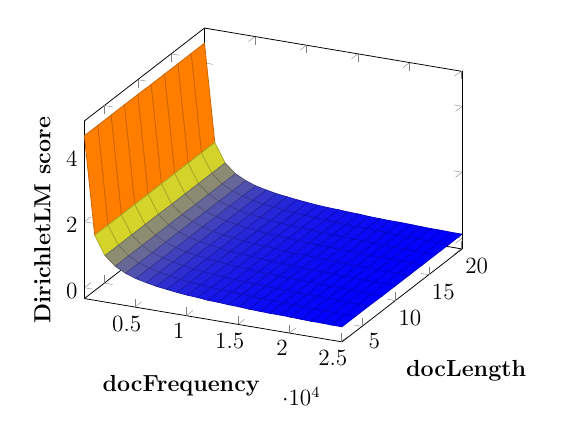
\begin{tikzpicture}[thick,scale=0.7, every node/.style={transform shape}] \begin{axis}[
 %title={},
 %y dir=reverse, 
 %x dir=reverse, 
 ylabel={docLength},
 xlabel={docFrequency},
 zlabel={DirichletLM score},
 every axis/.append style={font=\large\bfseries},
 max space between ticks=25pt
% yticklabels={0k,100k}
 ] 

		\addplot3[surf] coordinates { 
%patch,patch type=biquadratic, shader=faceted,patch refines=3
(100.00,20.00,4.60)(100.00,18.00,4.60)(100.00,16.00,4.60)(100.00,14.00,4.60)(100.00,12.00,4.60)(100.00,10.00,4.61)(100.00,8.00,4.61)(100.00,6.00,4.61)(100.00,4.00,4.61)(100.00,2.00,4.61)

(1100.00,20.00,1.64)(1100.00,18.00,1.64)(1100.00,16.00,1.64)(1100.00,14.00,1.64)(1100.00,12.00,1.64)(1100.00,10.00,1.64)(1100.00,8.00,1.64)(1100.00,6.00,1.64)(1100.00,4.00,1.64)(1100.00,2.00,1.65)

(2100.00,20.00,1.07)(2100.00,18.00,1.07)(2100.00,16.00,1.07)(2100.00,14.00,1.07)(2100.00,12.00,1.07)(2100.00,10.00,1.08)(2100.00,8.00,1.08)(2100.00,6.00,1.08)(2100.00,4.00,1.08)(2100.00,2.00,1.08)

(3100.00,20.00,0.80)(3100.00,18.00,0.80)(3100.00,16.00,0.80)(3100.00,14.00,0.80)(3100.00,12.00,0.81)(3100.00,10.00,0.81)(3100.00,8.00,0.81)(3100.00,6.00,0.81)(3100.00,4.00,0.81)(3100.00,2.00,0.81)

(4100.00,20.00,0.64)(4100.00,18.00,0.64)(4100.00,16.00,0.64)(4100.00,14.00,0.64)(4100.00,12.00,0.65)(4100.00,10.00,0.65)(4100.00,8.00,0.65)(4100.00,6.00,0.65)(4100.00,4.00,0.65)(4100.00,2.00,0.65)

(5100.00,20.00,0.53)(5100.00,18.00,0.54)(5100.00,16.00,0.54)(5100.00,14.00,0.54)(5100.00,12.00,0.54)(5100.00,10.00,0.54)(5100.00,8.00,0.54)(5100.00,6.00,0.54)(5100.00,4.00,0.54)(5100.00,2.00,0.54)

(6100.00,20.00,0.46)(6100.00,18.00,0.46)(6100.00,16.00,0.46)(6100.00,14.00,0.46)(6100.00,12.00,0.46)(6100.00,10.00,0.46)(6100.00,8.00,0.46)(6100.00,6.00,0.47)(6100.00,4.00,0.47)(6100.00,2.00,0.47)

(7100.00,20.00,0.40)(7100.00,18.00,0.40)(7100.00,16.00,0.40)(7100.00,14.00,0.40)(7100.00,12.00,0.40)(7100.00,10.00,0.41)(7100.00,8.00,0.41)(7100.00,6.00,0.41)(7100.00,4.00,0.41)(7100.00,2.00,0.41)

(8100.00,20.00,0.36)(8100.00,18.00,0.36)(8100.00,16.00,0.36)(8100.00,14.00,0.36)(8100.00,12.00,0.36)(8100.00,10.00,0.36)(8100.00,8.00,0.36)(8100.00,6.00,0.36)(8100.00,4.00,0.36)(8100.00,2.00,0.37)

(9100.00,20.00,0.32)(9100.00,18.00,0.32)(9100.00,16.00,0.32)(9100.00,14.00,0.32)(9100.00,12.00,0.32)(9100.00,10.00,0.32)(9100.00,8.00,0.33)(9100.00,6.00,0.33)(9100.00,4.00,0.33)(9100.00,2.00,0.33)

(10100.00,20.00,0.29)(10100.00,18.00,0.29)(10100.00,16.00,0.29)(10100.00,14.00,0.29)(10100.00,12.00,0.29)(10100.00,10.00,0.30)(10100.00,8.00,0.30)(10100.00,6.00,0.30)(10100.00,4.00,0.30)(10100.00,2.00,0.30)

(11100.00,20.00,0.26)(11100.00,18.00,0.27)(11100.00,16.00,0.27)(11100.00,14.00,0.27)(11100.00,12.00,0.27)(11100.00,10.00,0.27)(11100.00,8.00,0.27)(11100.00,6.00,0.27)(11100.00,4.00,0.27)(11100.00,2.00,0.28)

(12100.00,20.00,0.24)(12100.00,18.00,0.25)(12100.00,16.00,0.25)(12100.00,14.00,0.25)(12100.00,12.00,0.25)(12100.00,10.00,0.25)(12100.00,8.00,0.25)(12100.00,6.00,0.25)(12100.00,4.00,0.25)(12100.00,2.00,0.25)

(13100.00,20.00,0.23)(13100.00,18.00,0.23)(13100.00,16.00,0.23)(13100.00,14.00,0.23)(13100.00,12.00,0.23)(13100.00,10.00,0.23)(13100.00,8.00,0.23)(13100.00,6.00,0.23)(13100.00,4.00,0.24)(13100.00,2.00,0.24)

(14100.00,20.00,0.21)(14100.00,18.00,0.21)(14100.00,16.00,0.21)(14100.00,14.00,0.21)(14100.00,12.00,0.21)(14100.00,10.00,0.22)(14100.00,8.00,0.22)(14100.00,6.00,0.22)(14100.00,4.00,0.22)(14100.00,2.00,0.22)

(15100.00,20.00,0.20)(15100.00,18.00,0.20)(15100.00,16.00,0.20)(15100.00,14.00,0.20)(15100.00,12.00,0.20)(15100.00,10.00,0.20)(15100.00,8.00,0.20)(15100.00,6.00,0.20)(15100.00,4.00,0.21)(15100.00,2.00,0.21)

(16100.00,20.00,0.18)(16100.00,18.00,0.19)(16100.00,16.00,0.19)(16100.00,14.00,0.19)(16100.00,12.00,0.19)(16100.00,10.00,0.19)(16100.00,8.00,0.19)(16100.00,6.00,0.19)(16100.00,4.00,0.19)(16100.00,2.00,0.19)

(17100.00,20.00,0.17)(17100.00,18.00,0.18)(17100.00,16.00,0.18)(17100.00,14.00,0.18)(17100.00,12.00,0.18)(17100.00,10.00,0.18)(17100.00,8.00,0.18)(17100.00,6.00,0.18)(17100.00,4.00,0.18)(17100.00,2.00,0.18)

(18100.00,20.00,0.16)(18100.00,18.00,0.17)(18100.00,16.00,0.17)(18100.00,14.00,0.17)(18100.00,12.00,0.17)(18100.00,10.00,0.17)(18100.00,8.00,0.17)(18100.00,6.00,0.17)(18100.00,4.00,0.17)(18100.00,2.00,0.17)

(19100.00,20.00,0.16)(19100.00,18.00,0.16)(19100.00,16.00,0.16)(19100.00,14.00,0.16)(19100.00,12.00,0.16)(19100.00,10.00,0.16)(19100.00,8.00,0.16)(19100.00,6.00,0.16)(19100.00,4.00,0.16)(19100.00,2.00,0.17)

(20100.00,20.00,0.15)(20100.00,18.00,0.15)(20100.00,16.00,0.15)(20100.00,14.00,0.15)(20100.00,12.00,0.15)(20100.00,10.00,0.15)(20100.00,8.00,0.15)(20100.00,6.00,0.16)(20100.00,4.00,0.16)(20100.00,2.00,0.16)

(21100.00,20.00,0.14)(21100.00,18.00,0.14)(21100.00,16.00,0.14)(21100.00,14.00,0.14)(21100.00,12.00,0.15)(21100.00,10.00,0.15)(21100.00,8.00,0.15)(21100.00,6.00,0.15)(21100.00,4.00,0.15)(21100.00,2.00,0.15)

(22100.00,20.00,0.13)(22100.00,18.00,0.14)(22100.00,16.00,0.14)(22100.00,14.00,0.14)(22100.00,12.00,0.14)(22100.00,10.00,0.14)(22100.00,8.00,0.14)(22100.00,6.00,0.14)(22100.00,4.00,0.14)(22100.00,2.00,0.14)

(23100.00,20.00,0.13)(23100.00,18.00,0.13)(23100.00,16.00,0.13)(23100.00,14.00,0.13)(23100.00,12.00,0.13)(23100.00,10.00,0.13)(23100.00,8.00,0.13)(23100.00,6.00,0.14)(23100.00,4.00,0.14)(23100.00,2.00,0.14)

(24100.00,20.00,0.12)(24100.00,18.00,0.12)(24100.00,16.00,0.12)(24100.00,14.00,0.13)(24100.00,12.00,0.13)(24100.00,10.00,0.13)(24100.00,8.00,0.13)(24100.00,6.00,0.13)(24100.00,4.00,0.13)(24100.00,2.00,0.13)

(25100.00,20.00,0.12)(25100.00,18.00,0.12)(25100.00,16.00,0.12)(25100.00,14.00,0.12)(25100.00,12.00,0.12)(25100.00,10.00,0.12)(25100.00,8.00,0.12)(25100.00,6.00,0.13)(25100.00,4.00,0.13)(25100.00,2.00,0.13)

}; \end{axis} \end{tikzpicture}

          \label{dlmproof}          
        \end{subfigure}

        \caption{DLM evaluation figures}
\end{figure}

Figures \ref{dlmproofc2} and \ref{dlmproofcc} show DLM scores in terms of the $\mu$ parameter, w.r.t. document frequency and document length respectively. Figure \ref{dlmproof} on the other hand demonstrates the relation between document frequency and document length.

As we can observe from Equation \ref{dlmequation} the parameter $\mu$ is closely related to the collection statistics, and the length normalization component of the equation. Moreover the lower the values of $\mu$ the higher the score differences for similar document frequencies as shown in Figure \ref{dlmproofc2}. Similarly, we can observe in Figure \ref{dlmproofcc} how $\mu$ interacts with document length. For low values of $\mu$ we can observe how the scores are reduced at the same time that documents become larger, as expected for normal documents. Interestingly, this behaviour is dampened with higher values of $\mu$, as score differences are heavily reduced w.r.t. the different document lengths. Since the default value for $\mu$ is 2500, it is no surprise that document length has virtually no effect over the scores for DLM as seen in Figure \ref{dlmproof}, contrary to other retrieval models. 

\begin{table}[]

	\caption{P@30 scores for DLM for a range of $\mu$ values (All collections together)}
	\centering
	\begin{tabular}{l|c} 	
	\textit{\textbf{$\mu$}} & 
	\textit{\textbf{P@30}} 	
	\tabularnewline
	\hline
	1 & 0.4028 \\
	5 &  0.4164 \\
	20 & 0.4241 \\
	50 &  0.4099 \\
	100 &  0.3933 \\
	500 &  0.3396 \\
	1000 & 0.3227 \\
	2500 & 0.2988 \\
	\hline	
	\end{tabular}
	\label{drmmuvalues}
\end{table}

This could be a desired feature for microblog retrieval, however let us look at the performance achieved for a range of $\mu$ values in Table \ref{drmmuvalues}. As we can observe generally the higher the value of $mu$ the worse the performance obtained, with the exception of $\mu$ within the 1 to 20 range. 

In order to further understand the behaviour of DLM in the case of Microblog retrieval, we perform an analogous experiment to the previously performed for HLM. Since DLM was also designed for longer documents than microblogs, offsetting the statistics of TF and DL can be interesting experiment as it would better resemble its standard behaviour in term of the numerical values produced as scores. 

The results of the evaluation are presented in Table \ref{drmdtfmuvalues}. The first four lines contain the P@30 values for different combinations where $\mu$ is set to 20. As we can observe offsetting TF by +20 results in a substantial +7.47\% increase of P@30 with respect to the default configuration. On the other hand offsetting DL by +20 results in a 8.02\% decrease of performance in terms of P@30. Finally, combining the offsetting of both TF and DL results in comparable performance than that obtained by only increasing TF.

\begin{table}[]
	\caption{P@30 scores for DLM as we consider different combinations of dTF and dDL, and $\mu$, (All collections together)}
	\centering
	\begin{tabular}{l|c|c|c|c} 	
	&
	\textit{\textbf{$\mu$}} & 
	\textit{\textbf{dTF}} & 
	\textit{\textbf{dDL}} & 
	\textit{\textbf{P@30}} 	
	\tabularnewline
	\hline
	1 & 20 &    &    & 0.4241\\
	2 & 20 & 20 &    & 0.4558\\
	3 & 20 &    & 20 & 0.3901\\
	4 & 20 & 20 & 20 & 0.4547\\
	\hline	
	\hline
	5 & 2500 &    &    & 0.2988\\
	6 & 2500 & 20 &    & 0.4468\\
	7 & 2500 &    & 20 & 0.2892\\
	8 & 2500 & 20 & 20 & 0.4466\\
    \hline
	\end{tabular}
	\label{drmdtfmuvalues}
\end{table}

The same behaviour is obtained across all combinations when we set the $\mu = 2500$. To further develop our understanding of the behaviour, and to draw conclusions for such results, we devised Figures \ref{dlmfigureTFDL2500} and \ref{dlmfigureTFDL20}. Figures \ref{dlmfigureTFDL2500} and \ref{dlmfigureTFDL20} present the DLM scores produced with respect to Doc. Length (DL) and Term Frequency (TF) when $\mu=2500$ and $\mu=20$ respectively.

Let us analyse the results from Table \ref{drmdtfmuvalues} in connection with Figures \ref{dlmfigureTFDL2500} and \ref{dlmfigureTFDL20}. As we can observe incrementing DL will result in an increased differentiation of DLM scores with respect to TF as more values are closer to the minimum and maximum values. In other words there are less intermediate values (Light coloured areas), which ultimately reflects on heightened sensitivity to differences across the TF spectrum. Furthermore, we can also observe in Table \ref{drmdtfmuvalues} how incrementing DL values, results in worse performance in all cases. Consequently the increased differentiation of DLM scores with respect to the TF parameter, produced by the increment of DL is detrimental and in line with the findings in the previous section.

Additionally, Figure \ref{dlmfigureTFDL2500} shows an almost linear progression of DLM scores with respect to TF, whereas Figure \ref{dlmfigureTFDL20} ($\mu=20$) exhibits a logarithmic behaviour with respect to TF. The latter behaviour is more desirable because there should be a saturation point when incrementing TF at which there is very little value added to the score of the document, or could be even counter productive. In fact, if we take into consideration that term frequencies within microblogs are in the range 1-2, the pivoting value w.r.t TF should be very low, to avoid promoting spam microblogs.

The better behaviour with respect to TF is rewarded with increased performance whether the value of $\mu$ is 20 or 2500. In fact the offsetting of TF seems to overrule the effects of $\mu$ as similar results are obtained in both $\mu=20$ and $\mu=2500$ conditions. The effects of offsetting TF are most visually evident when looking at Figure \ref{dlmfigureTFDL20} as differences amongst the different scores become very small, when $TF > 20$. 


\begin{figure}
      	\begin{subfigure}[b]{0.5\textwidth}
          \centering
          \caption{Doc. length (DL) and Term Frequency (TF) when $\mu = 2500$}
          \input{dlmfigureTFDL2500}
          \label{dlmfigureTFDL2500}          
        \end{subfigure} 
        ~
 		\begin{subfigure}[b]{0.5\textwidth}
          \centering
          \caption{Doc. length (DL) and Term Frequency (TF) when $\mu = 20$}
          \input{dlmfigureTFDL}
          \label{dlmfigureTFDL20}          
        \end{subfigure} 
        \caption{Evaluating DLM's behaviour}
\end{figure}

Extending on the findings by \cite{naveed2011searching} who showed how length normalization was detrimental to microblog retrieval in an L2R retrieval framework. Our experiments have so far indicated the existence of a particular relationship between TF and DL that is most appropriate for Microblog retrieval. We believe that the score progressions with respect to \textit{DL should modelled by a very gentle slope}, whereas there should be a pivoting point with respect to \textit{TF where scores should decay} in order to account for spam. In the following sections these ideas will be further elaborated.

\subsection{The DFRee Case}
DFRee\footnote{http://terrier.org/docs/v2.2.1/javadoc/uk/ac/gla/terrier/matching/models/DFRee.html} is a Divergence From Randomness model implemented in the Terrier IR platform \cite{terrierir}. DFRee has been designed as a parameter-free model and adheres to the following implementation:

\begin{equation}
prior = \frac{f(q_i, D)}{|D|}, posterior = \frac{f(q_i, D)+1}{|D|+1} 
\end{equation}

\begin{equation}
InvPriorColl = \frac{ntoks}{f(q_i, C)}, norm = f(q_i, D)*log_2{\frac{posterior}{prior}}
\end{equation}

%\begin{equation}
\begin{multline}
DFRee(q_i,D,C) = norm * [                    \\
f(q_i, D)*(-log_2(prior*InvPriorColl))       \\
+(f(q_i, D)+1)*log_2(posterior*InvPriorColl) \\
+ 0.5*log_2(posterior/prior)],
\end{multline}

where \(f(q_i, D)\) represents the frequency of query term \(q_i\) within document \(D\). Similarly \(f(q_i, C)\) holds the collection \(C\) frequency for query term \(q_i\). Furthermore \(ntoks\) is the total number of unique terms within collection \(C\) and \(|D|\) represents the document length of document \(D\).

\begin{figure}
	\centering
	\caption{Evaluating DFR's behaviour: Doc. length (DL) and Term Frequency (TF)}
	%!TEX root = ./JournalChapter1.tex
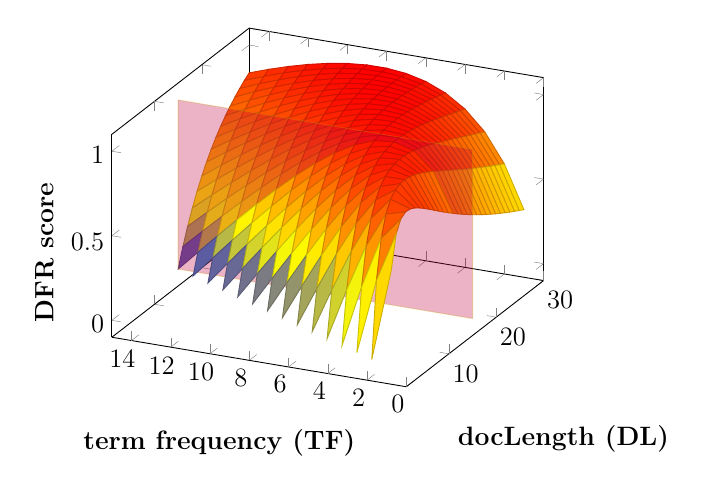
\begin{tikzpicture}[thick,scale=0.8, every node/.style={transform shape}]\begin{axis}[
 %title={},
% y dir=reverse, 
 x dir=reverse, 
 ylabel={docLength (DL)},
 xlabel={term frequency (TF)},
 zlabel={DFR score},
 every axis/.append style={font=\large\bfseries},
 max space between ticks=25pt
% yticklabels={0k,100k}
 ] 


\addplot3[surf,unbounded coords=jump]
coordinates  { 
(1,15,0.602828690204566)	(2,15,0.830458458727289)	(3,15,0.934450716638443)	(4,15,0.966903402267895)	(5,15,0.953929912325151)	(6,15,0.910204250164967)	(7,15,0.844773148573639)	(8,15,0.763616521737829)	(9,15,0.670903438148194)	(10,15,0.569664557459257)	(11,15,0.462178197338477)	(12,15,0.350204856834806)	(13,15,0.235136442615999)	(14,15,0.11809496699829)	(15,15,0)

(1,16,0.578099188538087)	(2,16,0.811155500645937)	(3,16,0.92455241464552)	(4,16,0.967767908505993)	(5,16,0.966062841257201)	(6,16,0.933720545287019)	(7,16,0.87957150961847)	(8,16,0.809460625419414)	(9,16,0.72746535973258)	(10,16,0.636550382771426)	(11,16,0.538944280996693)	(12,16,0.436368745300519)	(13,16,0.330184550451496)	(14,16,0.221488171413441)	(15,16,0.111177842268355)

(1,17,0.554089938092192)	(2,17,0.791526910417312)	(3,17,0.913056948252712)	(4,17,0.965714873324416)	(5,17,0.973972028301543)	(6,17,0.951752192118292)	(7,17,0.907687908109167)	(8,17,0.847501039032133)	(9,17,0.775185911781543)	(10,17,0.693647497457941)	(11,17,0.60506951435267)	(12,17,0.51113872004729)	(13,17,0.413187919650668)	(14,17,0.312290682010694)	(15,17,0.209326130035835)

(1,18,0.530802801771364)	(2,18,0.771767857536177)	(3,18,0.900372831623677)	(4,18,0.961364141168104)	(5,18,0.978478269819011)	(6,18,0.965306243347949)	(7,18,0.930298335362267)	(8,18,0.879063614353843)	(9,18,0.815520463917971)	(10,18,0.742519493293841)	(11,18,0.662203670865781)	(12,18,0.576228097258246)	(13,18,0.485900278395978)	(14,18,0.392273096789813)	(15,18,0.296208439454882)

(1,19,0.508226789640423)	(2,19,0.752018863072771)	(3,19,0.886810317359786)	(4,19,0.955195710616974)	(5,19,0.980224486964259)	(6,19,0.975178213356986)	(7,19,0.948338450288501)	(8,19,0.905210288059222)	(9,19,0.849642347853426)	(10,19,0.784435449978092)	(11,19,0.711695334773675)	(12,19,0.633048243551952)	(13,19,0.549778660548279)	(14,19,0.462920673152469)	(15,19,0.373320528862043)

(1,20,0.48634303905334)	(2,20,0.7323812008066)	(3,20,0.872607218288516)	(4,20,0.947585137098897)	(5,20,0.97971952494445)	(6,20,0.98200290254851)	(7,20,0.962559939768004)	(8,20,0.926799408296809)	(9,20,0.878505521275719)	(10,20,0.820433262364011)	(11,20,0.754654182131245)	(12,20,0.682768072499512)	(13,20,0.606038355509857)	(14,20,0.525481948969255)	(15,20,0.441930831844985)

(1,21,0.465128061580168)	(2,21,0.712927637929877)	(3,21,0.857947247761062)	(4,21,0.93882895517277)	(5,21,0.97736988612122)	(6,21,0.986291533238511)	(7,21,0.973572063624968)	(8,21,0.944530636289626)	(9,21,0.902891730766613)	(10,21,0.851367936716025)	(11,21,0.791999256676888)	(12,21,0.726361125537109)	(13,21,0.655697602410148)	(14,21,0.581009843803962)	(15,21,0.503116746944407)

(1,22,0.444555871588363)	(2,22,0.69371003859671)	(3,22,0.842973247656932)	(4,22,0.929163209859617)	(5,22,0.973503053852954)	(6,22,0.988459253367945)	(7,22,0.981872662054963)	(8,22,0.958978737875236)	(9,22,0.923446336219237)	(10,22,0.877948672683593)	(11,22,0.824496515075059)	(12,22,0.764642770856045)	(13,22,0.699613620363273)	(14,22,0.630395687626556)	(15,22,0.557795822851653)

(1,23,0.424599383032406)	(2,23,0.674764818583908)	(3,23,0.827796862032113)	(4,23,0.918777149915091)	(5,23,0.968384861977651)	(6,23,0.988845761863186)	(7,23,0.987871568720419)	(8,23,0.970619283566948)	(9,23,0.940705773382284)	(10,23,0.900767545813065)	(11,23,0.852788172693824)	(12,23,0.798299644283731)	(13,23,0.738511566834336)	(14,23,0.674397111108444)	(15,23,0.606751988315705)

(1,24,0.40523132186617)	(2,24,0.656116904788573)	(3,24,0.812505700538763)	(4,24,0.907823472234563)	(5,24,0.962232586378857)	(6,24,0.987730954630336)	(7,24,0.991908481950635)	(8,24,0.979848390893796)	(9,24,0.955118795248774)	(10,24,0.920321862204126)	(11,24,0.87741577498763)	(12,24,0.827913032165606)	(13,24,0.773007819631001)	(14,24,0.713660808324183)	(15,24,0.650657372038589)

(1,25,0.38642481493876)	(2,25,0.637782639637063)	(3,25,0.79716870357892)	(4,25,0.896426073240635)	(5,25,0.955224921679465)	(6,25,0.985346919947008)	(7,25,0.994266744020595)	(8,25,0.986998033599149)	(9,25,0.96706304333111)	(10,25,0.937031713492213)	(11,25,0.898838449553016)	(12,25,0.853977527193232)	(13,25,0.803628737708457)	(14,25,0.748741099129492)	(15,25,0.690090359300742)

(1,26,0.36815376139952)	(2,26,0.619771931399019)	(3,26,0.781840202366091)	(4,26,0.884685975052332)	(5,26,0.947509661773085)	(6,26,0.981887225781465)	(7,26,0.995184065634633)	(8,26,0.992348018723311)	(9,26,0.976858081971228)	(10,26,0.95125386482836)	(11,26,0.917447437797707)	(12,26,0.876915988605277)	(13,26,0.830825830481115)	(14,26,0.78011508458774)	(15,26,0.725550507465349)

(1,27,0.350393057325973)	(2,27,0.60208985927249)	(3,27,0.766563020474647)	(4,27,0.872685899583419)	(5,27,0.939209668327629)	(6,27,0.977514176161289)	(7,27,0.994860946200371)	(8,27,0.996135435044116)	(9,27,0.984775730704953)	(10,27,0.963292820489072)	(11,27,0.933577738074063)	(12,27,0.897091603060034)	(13,27,0.854988073305192)	(14,27,0.808195051131356)	(15,27,0.757470870504045)

(1,28,0.333118721214438)	(2,28,0.584737880102515)	(3,28,0.751370863683325)	(4,28,0.860493830168551)	(5,28,0.930427549263709)	(6,28,0.97236452885122)	(7,28,0.993467339157226)	(8,28,0.998562165131648)	(9,28,0.99104831536007)	(10,28,0.973409701227053)	(11,28,0.947517492491807)	(12,28,0.914817660899949)	(13,28,0.876451950536151)	(14,28,0.833338655534655)	(15,28,0.786228199121581)

(1,29,0.316307952698114)	(2,29,0.567714741253384)	(3,29,0.736290176025056)	(4,29,0.848165807395434)	(5,29,0.921249355632251)	(6,29,0.966554036195814)	(7,29,0.991147968519457)	(8,29,0.999800901797173)	(9,29,0.995875303197284)	(10,29,0.981829412799183)	(11,29,0.959515600327343)	(12,29,0.930365523362214)	(13,29,0.89550968334361)	(14,29,0.855857318363783)	(15,29,0.81215140336571)

(1,30,0.299939146627551)	(2,30,0.55101717484961)	(3,30,0.721341591745516)	(4,30,0.835748140323265)	(5,30,0.911747524748403)	(6,30,0.960181077894388)	(7,30,0.988026599941357)	(8,30,1)	(9,30,0.999428673828312)	(10,30,0.98874647076145)	(11,30,0.969787928978429)	(12,30,0.943971149900242)	(13,30,0.912416001900636)	(14,30,0.876023168107538)	(15,30,0.835528594560206)

};

\addplot3 [data cs=cart,surf,domain=-10:10,samples=2, opacity=0.3,color=purple] coordinates  { 
(0,15,0) (0,15,1)

(15,15,0) (15,15,1)

};


\addplot3[surf,unbounded coords=jump]
coordinates  { 
%patch,patch type=biquadratic, shader=faceted,patch refines=3
(1,1,0)	(2,1,nan)	(3,1,nan)	(4,1,nan)	(5,1,nan)	(6,1,nan)	(7,1,nan)	(8,1,nan)	(9,1,nan)	(10,1,nan)	(11,1,nan)	(12,1,nan)	(13,1,nan)	(14,1,nan)	(15,1,nan)

(1,2,0.550946811011921)	(2,2,0)	(3,2,nan)	(4,2,nan)	(5,2,nan)	(6,2,nan)	(7,2,nan)	(8,2,nan)	(9,2,nan)	(10,2,nan)	(11,2,nan)	(12,2,nan)	(13,2,nan)	(14,2,nan)	(15,2,nan)

(1,3,0.739499035509737)	(2,3,0.447402531994322)	(3,3,0)	(4,3,nan)	(5,3,nan)	(6,3,nan)	(7,3,nan)	(8,3,nan)	(9,3,nan)	(10,3,nan)	(11,3,nan)	(12,3,nan)	(13,3,nan)	(14,3,nan)	(15,3,nan)

(1,4,0.808372355369359)	(2,4,0.674021740218476)	(3,4,0.367084989657738)	(4,4,0)	(5,4,nan)	(6,4,nan)	(7,4,nan)	(8,4,nan)	(9,4,nan)	(10,4,nan)	(11,4,nan)	(12,4,nan)	(13,4,nan)	(14,4,nan)	(15,4,nan)

(1,5,0.827712304044469)	(2,5,0.795475244633043)	(3,5,0.589020399660793)	(4,5,0.309402318963368)	(5,5,0)	(6,5,nan)	(7,5,nan)	(8,5,nan)	(9,5,nan)	(10,5,nan)	(11,5,nan)	(12,5,nan)	(13,5,nan)	(14,5,nan)	(15,5,nan)

(1,6,0.823758030119902)	(2,6,0.861291472386904)	(3,6,0.728208149339069)	(4,6,0.516703283500178)	(5,6,0.266826414784725)	(6,6,0)	(7,6,nan)	(8,6,nan)	(9,6,nan)	(10,6,nan)	(11,6,nan)	(12,6,nan)	(13,6,nan)	(14,6,nan)	(15,6,nan)

(1,7,0.808049149749894)	(2,7,0.895286730204683)	(3,7,0.81731608309985)	(4,7,0.659114482699154)	(5,7,0.458088606324659)	(6,7,0.234329891272407)	(7,7,0)	(8,7,nan)	(9,7,nan)	(10,7,nan)	(11,7,nan)	(12,7,nan)	(13,7,nan)	(14,7,nan)	(15,7,nan)

(1,8,0.786232834510155)	(2,8,0.910031065751261)	(3,8,0.874547067067584)	(4,8,0.758685635473427)	(5,8,0.597677806310571)	(6,8,0.410536626837436)	(7,8,0.208787788218013)	(8,8,0)	(9,8,nan)	(10,8,nan)	(11,8,nan)	(12,8,nan)	(13,8,nan)	(14,8,nan)	(15,8,nan)

(1,9,0.761283776662586)	(2,9,0.912649127410629)	(3,9,0.9106548363097)	(4,9,0.828974496924382)	(5,9,0.700999123980372)	(6,9,0.54484240060699)	(7,9,0.371505245812937)	(8,9,0.188214411477962)	(9,9,0)	(10,9,nan)	(11,9,nan)	(12,9,nan)	(13,9,nan)	(14,9,nan)	(15,9,nan)

(1,10,0.734851414275236)	(2,10,0.907408307407578)	(3,10,0.932312475346719)	(4,10,0.878648510130617)	(5,10,0.778218625288615)	(6,10,0.648369486864792)	(7,10,0.499658763815525)	(8,10,0.339026534140879)	(9,10,0.171302777785929)	(10,10,0)	(11,10,nan)	(12,10,nan)	(13,10,nan)	(14,10,nan)	(15,10,nan)

(1,11,0.707882534208275)	(2,11,0.896978134982265)	(3,11,0.943832686982997)	(4,11,0.91344706582647)	(5,11,0.83622890765175)	(6,11,0.728859016655641)	(7,11,0.601513634159584)	(8,11,0.460887857152159)	(9,11,0.311641587291567)	(10,11,0.157162472776661)	(11,11,0)	(12,11,nan)	(13,11,nan)	(14,11,nan)	(15,11,nan)

(1,12,0.680931777320597)	(2,12,0.883087512447978)	(3,12,0.948098319824685)	(4,12,0.937288690029642)	(5,12,0.879825806210446)	(6,12,0.791804036576653)	(7,12,0.683066380350784)	(8,12,0.560095278476284)	(9,12,0.427403757686762)	(10,12,0.288272090676837)	(11,12,0.145167857760471)	(12,12,0)	(13,12,nan)	(14,12,nan)	(15,12,nan)

(1,13,0.654326072191879)	(2,13,0.866887863527846)	(3,13,0.947091556647468)	(4,13,0.95292023017884)	(5,13,0.912425568445965)	(6,13,0.841179268774445)	(7,13,0.748729504809226)	(8,13,0.641371703296107)	(9,13,0.523490353484945)	(10,13,0.398272129069081)	(11,13,0.268113442610775)	(12,13,0.134867288166317)	(13,13,0)	(14,13,nan)	(15,13,nan)

(1,14,0.628256015834611)	(2,14,0.849163506028517)	(3,14,0.942208095803169)	(4,14,0.962311537733073)	(5,14,0.936513154948686)	(6,14,0.879914128436669)	(7,14,0.80179902209063)	(8,14,0.708296983893924)	(9,14,0.603678740961905)	(10,14,0.491048437946633)	(11,14,0.372739929982426)	(12,14,0.25055715796921)	(13,14,0.125926946814904)	(14,14,0)	(15,14,nan)

(1,15,0.602828690204566)	(2,15,0.830458458727289)	(3,15,0.934450716638443)	(4,15,0.966903402267895)	(5,15,0.953929912325151)	(6,15,0.910204250164967)	(7,15,0.844773148573639)	(8,15,0.763616521737829)	(9,15,0.670903438148194)	(10,15,0.569664557459257)	(11,15,0.462178197338477)	(12,15,0.350204856834806)	(13,15,0.235136442615999)	(14,15,0.11809496699829)	(15,15,0)

};


 \end{axis} \end{tikzpicture}

	\label{dfrTFDLcomp}
\end{figure} 

Similarly to the evaluations carried out in previous sections, we simulated the scores produced by DFRee given a range of TF and DL values. The objective is studying its behaviour in microbloging conditions, and draw conclusions about its performance. These simulated values are shown in Figure \ref{dfrTFDLcomp}.

As we traverse the Document Length axis we can observe an interesting behaviour which is not present in any model observed so far. 

For low values of TF, incrementing DL from 1 to $\sim16$ results in also a higher score. This behaviour aligns with the scope hypotheses as longer documents are regarded as more informative. However, when DL reaches high enough values the scores start to decline. The latter behaviour is in line with the verbose hypotheses which assumes the extra length is due to superfluous information. Particularly when the extended document length is not accompanied by higher query term frequencies.

When dealing with documents as short as microblogs it is very difficult to assert their informativeness or relevance in terms of the verbose or scope hypotheses. In fact all retrieval models observed so far follow these to some degree and perform worse than a simply using IDF as a retrieval model. Additionally, the premises in which they are built seem not to hold as they fail to perform better than simple IDF. However DFRee is an interesting exception as it performs better than all the studied retrieval models, and it performs better than IDF in some cases (Table \ref{traditional}).

We believe that the \textit{saturation point} observed in Figure \ref{dfrTFDLcomp} in terms of TF and DL is responsible for DFRee outperforming other retrieval models in this task (And sometimes IDF). The score produced by DFRee can only be higher if both TF and DL increase. Thus, incrementing the value of a single component will increase the score to a saturation point after which the score will then decrease. As an example, consider an average microblog document of length 15 (blue plane in Figure \ref{dfrTFDLcomp}). The score is maximised when TF approaches 3, after which higher TF values result in a significant reduction to the score.

This behaviour opposed to that of BM25, HLM and DLM which exhibit a positive correlation between TF and the score produced. Note that in this case a document made up of repeating query terms would be valued over others with richer, and more informative content. This behaviour is obviously problematic as it promotes spam-like documents. Fortunately DFRee has a pivoting point which attempts to alleviate this possibility, thus reducing the value of increasing TF in short documents.

Recall that users of microblog services such as Twitter, strive to fit their messages within the character limit. It stands to reason, that the more terms they fit within the character limit the higher the chances of it being informative. The pivoted behaviour of DFRee does not completely match this premise, however it does match it better than all other observed retrieval models (Including BM25, HLM and DLM) where longer documents are simply less relevant under microblog conditions.

Summarising, we believe that DFRee's behaviour is key to better understand why most retrieval models fail to capture the relevance of microblogs. Particularly important is the \textit{saturation point} behaviour as a function of TF and DL. We can observe that promoting documents that are longer, whilst penalising documents with higher TF values than 2 may be a better fit to capture microblogs' relevance.

\subsection{Harmonising Score differences}
So far we have introduced a set of representative retrieval models, and discussed how they behave when facing microblog-like conditions. We have mainly simulated the spectrum of scores produced w.r.t. TF and DL by each model when fixing all other parameters. Moreover we have observed that retrieval models performance seems to increase when we overestimate the values of TF and DL, thus forcing the models to return values of lesser score differences.


\begin{table}[]
	\caption{Behaviour when harmonising score differences.(All collections together.)}
	\centering
	\begin{tabular}{l|c|c|c} 	
		\textit{\textbf{Model}} & 
		\textit{\textbf{configuration}} & 
		\textit{\textbf{stdev}} & 
		\textit{\textbf{P@30}} 	
		\tabularnewline
		\hline
		DLM & \(c=2500\) & 0.2639 & 0.2988 \\
		DLM & \(c=50\) & 0.2479 & 0.4099 \\
		DLM & \(c=20\) & 0.2384 & 0.4241 \\
		\hline	
		HLM & \(c=0.15\) & 0.2553 & 0.3475\\
		HLM & \(c=0.40\) & 0.2365 & 0.4009\\
		HLM & \(c=0.99\) & 0.1135 & 0.4492\\
		\hline
		BM25 & \(b=0.75, k=1.2\) & 0.1274 & 0.3948\\
		BM25 & \(b=0.75, k=0.7\) & 0.0927 & 0.4399\\
		BM25 & \(b=0.9, k=0.1\) & 0.0181 & 0.4580\\
%		\hline
%		DFRee & NA & 0.2268 & 0.4614\\
		\hline
		\hline    
		PEARSON & \multicolumn{2}{|c}{-0.70}    \\ %(-0.58 including DFRee)
		KTau & \multicolumn{2}{|c}{-0.66}    \\ %(-0.56 including DFRee)
	\end{tabular}
	\label{stdevharmonising}
\end{table}

Table \ref{stdevharmonising} holds a summary of the results for all retrieval models with various configurations with respect to Precision@30. Additionally the third column holds the standard deviation of the simulated scores produced by the retrieval models in microblog conditions\footnote{where $DL<=30$ and $TF<=15$}. 

As it can be easily observed, the possible document scores are much closer together for those configurations that improve a retrieval model's performance. In fact there is a strong statistical correlation (last two columns) between reducing the standard deviation and improving the retrieval performance of the models. This observation motivates the following hypothesis:

\begin{quotation}
\begin{quote}
\textbf{The range of scores produced by retrieval models can be unfairly different due to its behaviour w.r.t. the scarcity of TF and DL values in microblog conditions.}
\end{quote}
\end{quotation}


If this hypothesis is true, we should be able to achieve similar positive results if we reduce the scoring differences of a retrieval model by means of any other technique. To this end we decided to apply a base two logarithm, to the scoring function of each retrieval model. As an example, the formulation of HLM would be as follows: 

\begin{small}
	\begin{align}
	\label{hlmformulalog}
	\text{HLM}(D,Q) &=  \sum_{i=1}^{n} \bf{log_2} \left[ \log_2 \left[ 1 + \frac{c \cdot f(q_i, D) \cdot ntoks }{ (1-c) \cdot f(q_i, C) \cdot |D|} \right] \right]
	\end{align}
\end{small}

\noindent where the added logarithm function can be found next to the summation sign.

Table \ref{loggedRMS} holds a comparison between the default P@30 achieved by each model and the same model with the log function applied to it. As we can observe the results for DLM, HLM and BM25 perform significantly better than their standard, whereas DFRee performs marginally worse and IDF remains unaffected.

From these experiments we can conclude that state of the art retrieval models produce unfair scores due to the scarcity of TF and DL during microblog retrieval. This effect can be mitigated by employing techniques to reduce possible score differences such as applying a log function. To conclude, when ranking microblog documents our models should consider the existing TF and DL evidence, but should also be conservative when managing the overall effects on the produced scores.
%
%\todo{We can conclude that based on this evidence most retrieval models are not prepared to effectively capture the relevance of microblogs. The verbose and scope hypotheses, which serves as inspiration to most retrieval models, do not hold for microblog documents. Additionally, the main reason points to their over-sensitiveness to low values of term frequency and document length. This sensitiveness often produces a high degree of score differences amongst the ranked documents which ultimately negatively affects performance.}

\begin{table}[]
	
	\caption{Retrieval models performance with log-smoothed scores (All collections)} 
	\centering
	\begin{tabular}{l|c|c|c|} 
		\multicolumn{1}{c}{}&\multicolumn{3}{|c|}{Precision @ 30} \\ 
		\cline{2- 4}
			& Default & $log_2(Ret. Model)$ & \% difference \\
		\hline
					 
		$DLM$ & 0.2988 & 0.3977 & +33.10\% \\
		$HLM$ & 0.3475 & 0.4489 & +29.18\%\\
		$BM25$ & 0.3948 & 0.4336 & +9.83\%\\
		$DFRee$ & 0.4614 & 0.4531 & -1.80\%\\
		$IDF$ & 0.4626 & 0.4626 & 0\%\\
		\hline
	\end{tabular}
	\label{loggedRMS}
\end{table}
